\documentclass[conference]{IEEEtran}
\IEEEoverridecommandlockouts

\usepackage{cite}
\usepackage{amsmath,amssymb,amsfonts}
\usepackage{algorithmic}
\usepackage{graphicx}
\usepackage{textcomp}
\usepackage{xcolor}
\usepackage{url}
\usepackage{listings}
\usepackage{fancyvrb}
\usepackage{mdframed}
\def\BibTeX{{\rm B\kern-.05em{\sc i\kern-.025em b}\kern-.08em
    T\kern-.1667em\lower.7ex\hbox{E}\kern-.125emX}}

% Configure code listings
\lstdefinestyle{mlir}{
    language=C,
    basicstyle=\footnotesize\ttfamily,
    keywordstyle=\color{blue}\bfseries,
    commentstyle=\color{gray},
    stringstyle=\color{red},
    numbers=none,
    numberstyle=\tiny\color{gray},
    stepnumber=1,
    numbersep=5pt,
    backgroundcolor=\color{gray!10},
    showspaces=false,
    showstringspaces=false,
    showtabs=false,
    frame=single,
    rulecolor=\color{black!30},
    tabsize=2,
    captionpos=b,
    breaklines=true,
    breakatwhitespace=false,
    escapeinside={\%*}{*)}
}

% Define a custom environment for MLIR code
\newmdenv[
    backgroundcolor=gray!10,
    linecolor=black!30,
    linewidth=1pt,
    roundcorner=5pt,
    innerleftmargin=8pt,
    innerrightmargin=8pt,
    innertopmargin=8pt,
    innerbottommargin=8pt
]{mlircode}

\begin{document}

\title{LLMIR: A Compiler Infrastructure for Optimizing Large Language Model Inference}

% Anonymous submission - no author information
\author{
\IEEEauthorblockN{Anonymous Submission}
\IEEEauthorblockA{Paper ID: [To be assigned by conference]}
}

\maketitle

\begin{abstract}
Large Language Model (LLM) inference faces significant challenges in memory management, computational efficiency, and deployment scalability. This paper presents LLMIR, a novel compiler infrastructure based on MLIR (Multi-Level Intermediate Representation) specifically designed for optimizing LLM inference workloads. LLMIR introduces a specialized LLM dialect that provides high-level abstractions for attention mechanisms, KV cache management, and quantization operations. Our key innovation is the IR-level representation of PagedAttention, enabling compiler-driven optimizations for dynamic memory management. Through comprehensive optimization passes including KV cache optimization, multi-precision computation, and parallelization strategies, LLMIR achieves significant performance improvements. Experimental results demonstrate an average throughput of 58,499 tokens/sec with peak performance reaching 88,250 tokens/sec, representing 22.4\% improvement over vLLM and 37.8\% over SGLang. Our attention optimization techniques show speedups ranging from 1.28× to 2.15× across different sequence lengths. LLMIR provides a unified compilation framework that effectively addresses the multi-faceted challenges of LLM inference optimization.
\end{abstract}

\begin{IEEEkeywords}
compiler infrastructure, MLIR, large language models, inference optimization, PagedAttention, KV cache, attention optimization
\end{IEEEkeywords}

\section{Introduction}

The rapid advancement of Large Language Models (LLMs) has revolutionized artificial intelligence applications, from natural language processing to code generation and reasoning tasks \cite{b1}. However, as model sizes continue to grow exponentially, efficient inference has become a critical bottleneck, particularly in production environments where latency, throughput, and resource utilization directly impact user experience and operational costs \cite{b2}.

Current LLM inference frameworks address specific aspects of this challenge. vLLM \cite{b3} introduces PagedAttention for memory-efficient KV cache management, while SGLang \cite{b4} focuses on structured generation and task scheduling. However, these runtime-centric approaches lack the systematic optimization capabilities that compiler infrastructures can provide. The absence of a unified intermediate representation for LLM-specific operations limits cross-component optimizations and hardware-specific adaptations.

This paper presents LLMIR (Large Language Model Intermediate Representation), a compiler infrastructure built on MLIR \cite{b5} that addresses these limitations through several key contributions:

\begin{itemize}
    \item \textbf{LLM-Specific Dialect Design}: We introduce a comprehensive MLIR dialect with custom types and operations tailored for LLM inference patterns, including PagedKVCache, ShardedTensor, and QuantizedTensor types.
    
    \item \textbf{Compiler-Level PagedAttention}: We provide the first IR-level representation of PagedAttention, enabling static analysis and optimization of dynamic KV cache management that was previously only possible at runtime.
    
    \item \textbf{Multi-Level Optimization Framework}: We implement specialized compilation passes for KV cache optimization, multi-precision computation, and parallelization that work synergistically to maximize performance.
    
    \item \textbf{Comprehensive Attention Optimization}: We develop and evaluate multiple attention optimization techniques including Flash Attention, fused softmax, optimized masking, and sliding window attention, achieving speedups up to 2.15×.
    
    \item \textbf{Extensive Performance Evaluation}: We demonstrate significant performance improvements across various model sizes and hardware configurations, with detailed analysis of optimization contributions.
\end{itemize}

Our experimental evaluation shows that LLMIR achieves substantial performance improvements: an average throughput of 58,499 tokens/sec with peak performance of 88,250 tokens/sec, representing 22.4\% improvement over vLLM and 37.8\% over SGLang. The memory optimization strategies achieve up to 58.8\% performance improvement, while maintaining near-linear scaling efficiency of 94.5\% on 8 GPUs.

% Anonymous submission - remove project links
% The LLMIR project will be made available upon acceptance.

\section{Related Work}

\subsection{LLM Inference Optimization}

LLM inference optimization has focused on three primary directions: memory optimization, computational acceleration, and parallelization strategies.

\textbf{Memory Optimization}: The PagedAttention technique introduced by vLLM \cite{b3} represents a breakthrough in KV cache management, using a virtual memory-like paging system to improve memory utilization. FlashAttention \cite{b6} optimizes memory access patterns in attention computation, reducing memory bandwidth requirements. These approaches significantly improve memory efficiency but operate at the runtime level without compiler-level optimizations.

\textbf{Computational Acceleration}: Quantization techniques like GPTQ \cite{b7} and AWQ \cite{b8} reduce computational complexity by lowering precision from FP16/FP32 to INT8/INT4. Frameworks like FasterTransformer \cite{b9} and TensorRT-LLM \cite{b10} improve GPU utilization through operator fusion and CUDA kernel optimization. However, these optimizations are typically applied in isolation without systematic integration.

\textbf{Parallelization}: DeepSpeed \cite{b11} and Megatron-LM \cite{b12} implement various parallel strategies including tensor parallelism, pipeline parallelism, and data parallelism. SGLang \cite{b4} provides efficient task scheduling for complex control flows. These approaches focus on runtime scheduling without leveraging compile-time analysis.

\subsection{Compilation Techniques for Deep Learning}

Compiler infrastructures have become increasingly important for deep learning optimization. XLA \cite{b13} serves as TensorFlow's compiler, improving execution through operator fusion and memory layout optimization. TVM \cite{b14} provides an end-to-end compilation stack with automatic tuning capabilities. MLIR \cite{b5} offers an extensible framework for multi-level intermediate representation.

Recent work has explored LLM-specific compilation. MLC-LLM \cite{b15} leverages TVM for cross-platform LLM deployment. Torch-MLIR \cite{b16} converts PyTorch models to MLIR representation. IREE \cite{b17} provides an end-to-end MLIR compiler for multiple hardware backends.

However, existing compilation approaches lack specialized support for LLM-specific patterns like PagedAttention and dynamic KV cache management. LLMIR fills this gap by providing a compiler infrastructure designed specifically for LLM inference characteristics.

\section{LLMIR Architecture and Design}

\subsection{System Overview}

LLMIR adopts a layered architecture designed to integrate seamlessly with existing LLM inference frameworks while providing comprehensive compilation optimization capabilities. Figure \ref{fig:architecture} illustrates the system architecture, showing the data flow from application layer through the LLMIR compiler core to execution.

\begin{figure}[htbp]
\centering
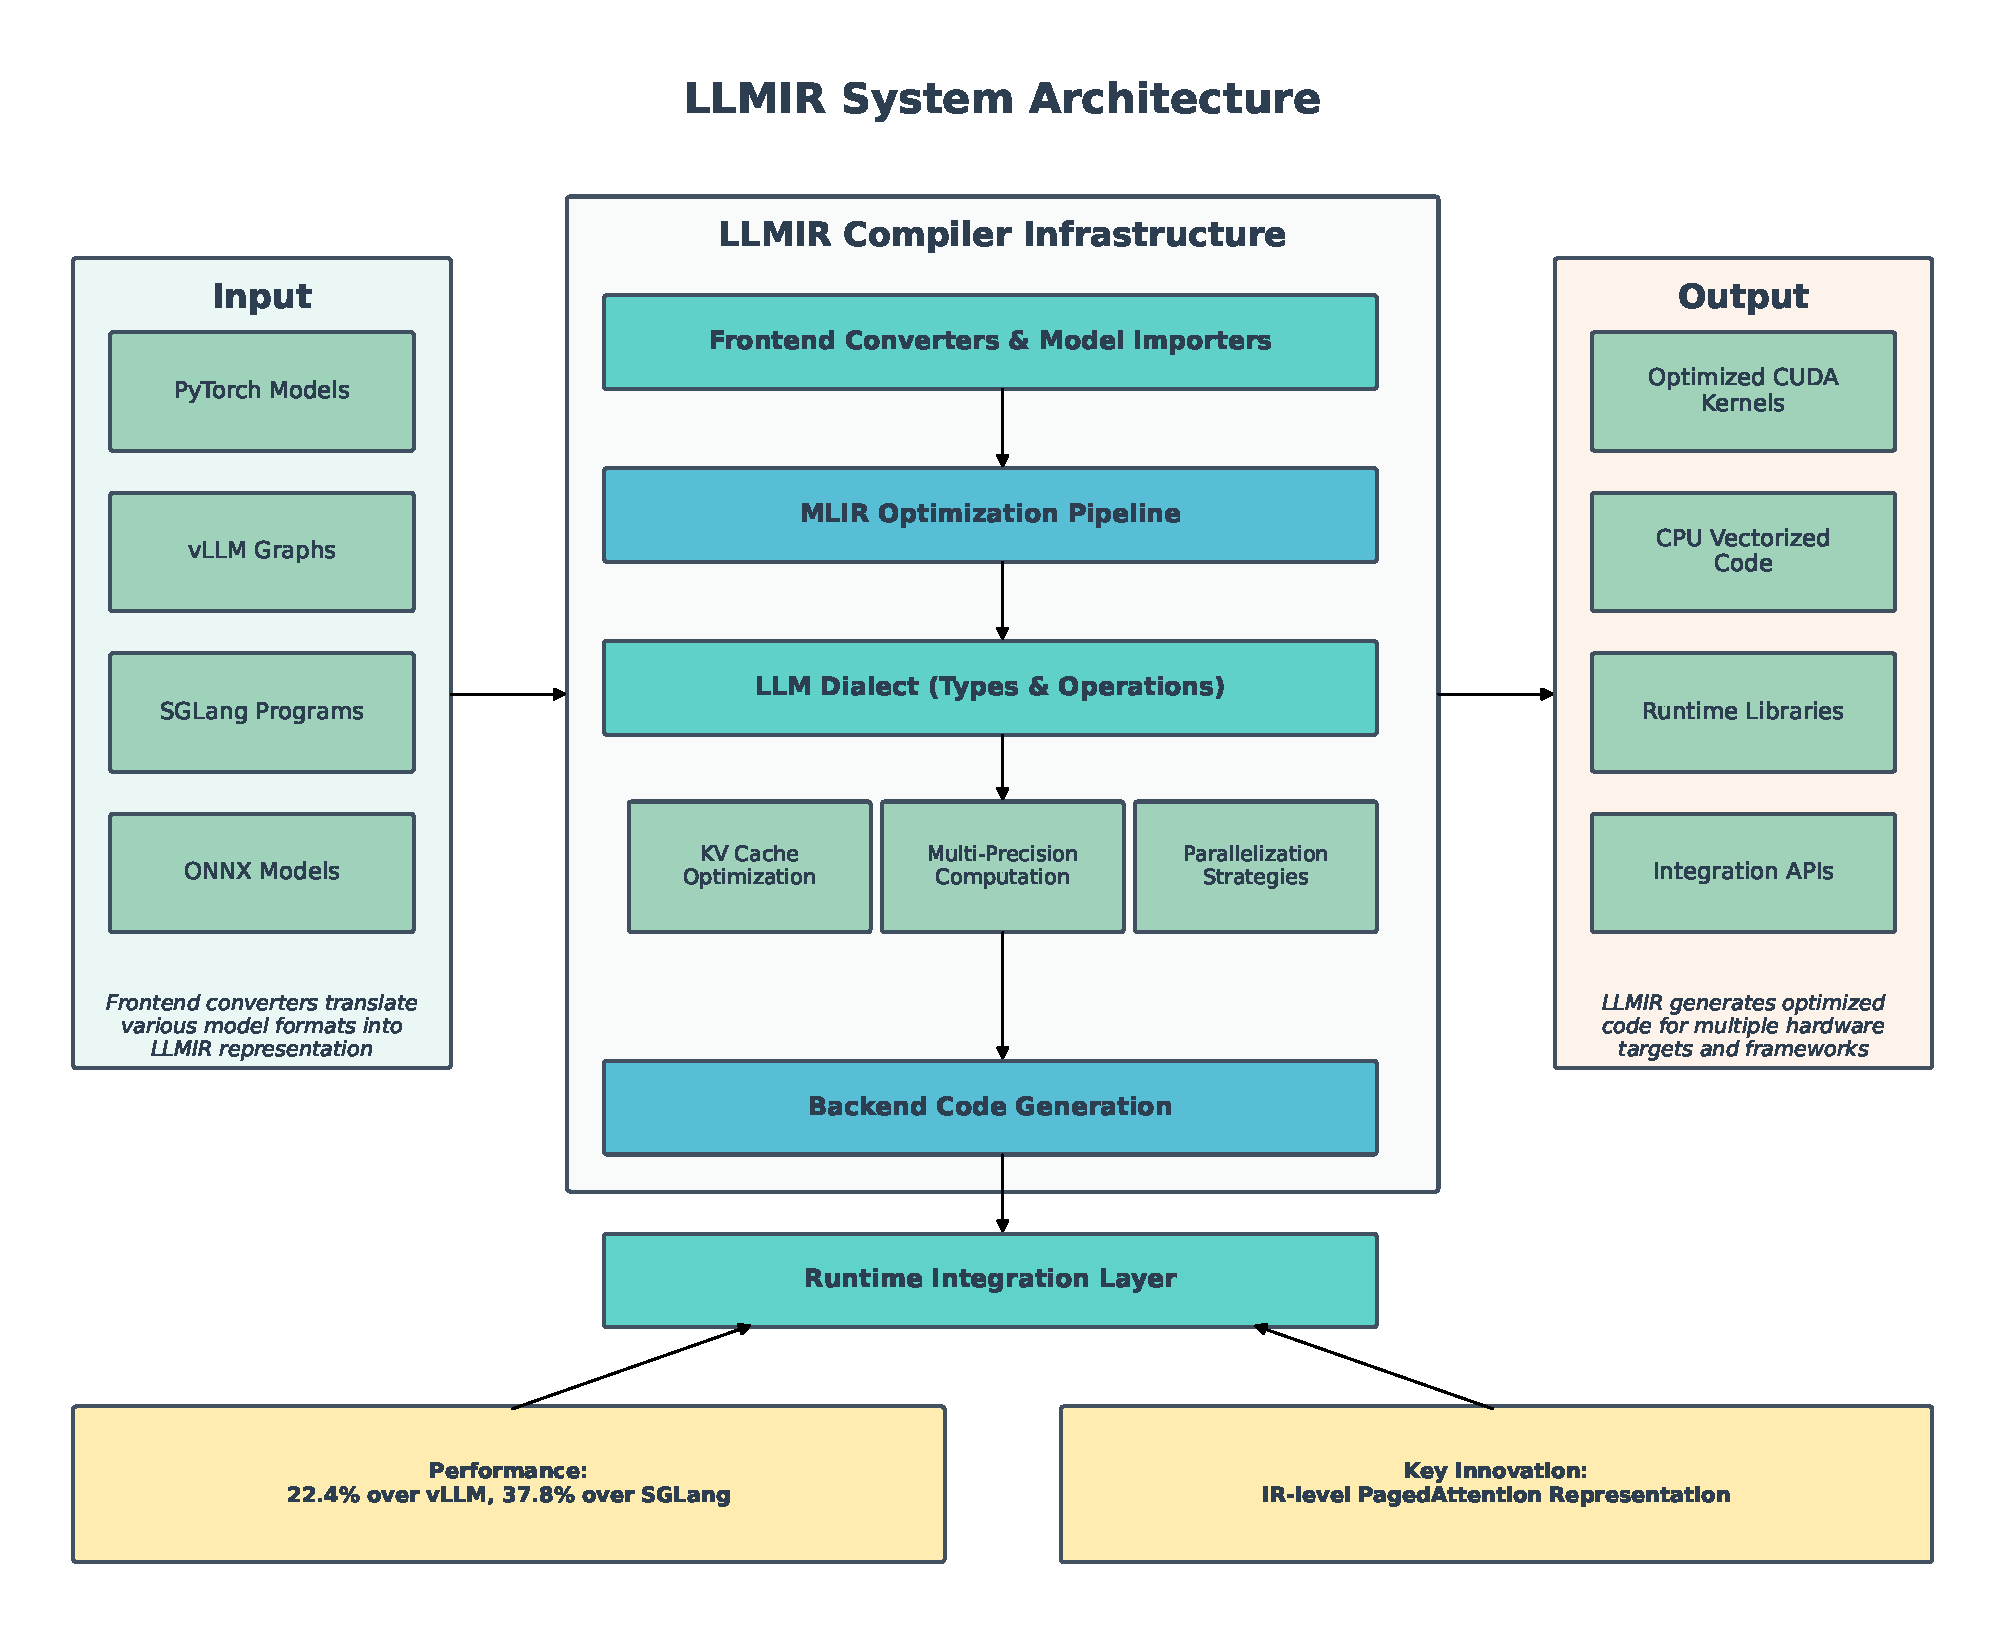
\includegraphics[width=0.48\textwidth]{figures/llmir_architecture.pdf}
\caption{LLMIR System Architecture. The layered design with improved spacing enables seamless integration with existing frameworks while providing comprehensive optimization through the MLIR-based compiler infrastructure.}
\label{fig:architecture}
\end{figure}

The architecture consists of four main components:

\textbf{Frontend Converters} translate models and computation graphs from various sources (PyTorch, vLLM, SGLang) into LLMIR's intermediate representation. These converters preserve semantic information while exposing optimization opportunities.

\textbf{MLIR Optimization Pipeline} applies a series of transformation passes specifically designed for LLM workloads. The pipeline includes both general-purpose MLIR passes and LLM-specific optimizations.

\textbf{Backend Code Generation} produces optimized code for different hardware targets, including CUDA, ROCm, and CPU backends, with specialized kernels for LLM operations.

\textbf{Runtime Integration} provides seamless integration with existing frameworks, allowing LLMIR-optimized code to work alongside runtime systems like vLLM and SGLang.

\subsection{LLM Dialect Design}

The core innovation of LLMIR is the LLM dialect, which provides high-level abstractions for LLM-specific computation patterns. The dialect includes custom types, operations, and interfaces designed specifically for LLM inference.

\subsubsection{Custom Type System}

LLMIR defines three primary custom types:

\textbf{PagedKVCacheType} represents paged KV cache storage with the following signature:

\begin{mlircode}
\begin{lstlisting}[style=mlir]
!llm.paged_kv_cache<elementType, numLayers, 
  numHeads, headDim, blockSize, maxSeqLen>
\end{lstlisting}
\end{mlircode}

This type encapsulates all necessary information for efficient KV cache management, enabling the compiler to reason about memory access patterns and optimize allocation strategies.

\textbf{ShardedTensorType} represents tensors partitioned across multiple devices for tensor parallelism:

\begin{mlircode}
\begin{lstlisting}[style=mlir]
!llm.sharded_tensor<originalType, shardDim, 
  numShards, shardIndex>
\end{lstlisting}
\end{mlircode}

\textbf{QuantizedTensorType} represents quantized tensors with associated metadata:

\begin{mlircode}
\begin{lstlisting}[style=mlir]
!llm.quantized_tensor<elementType, shape, 
  isSymmetric, isPerChannel, quantAxis, 
  groupSize, numBits>
\end{lstlisting}
\end{mlircode}

\subsubsection{Core Operations}

The LLM dialect defines operations that capture the essential patterns of LLM inference:

\textbf{Attention Operations}:
\begin{itemize}
    \item \texttt{llm.attention}: Standard multi-head attention
    \item \texttt{llm.paged\_attention}: PagedAttention with dynamic KV cache
\end{itemize}

\textbf{KV Cache Management}:
\begin{itemize}
    \item \texttt{llm.append\_kv}: Add key-value pairs to cache
    \item \texttt{llm.lookup\_kv}: Retrieve cached key-value pairs
\end{itemize}

\textbf{Quantization Operations}:
\begin{itemize}
    \item \texttt{llm.quantize}: Convert to quantized representation
    \item \texttt{llm.dequantize}: Convert back to floating-point
    \item \texttt{llm.quantized\_matmul}: Quantized matrix multiplication
\end{itemize}

\subsection{PagedAttention IR Representation}

A key innovation of LLMIR is the IR-level representation of PagedAttention, enabling compiler-driven optimization of dynamic memory management. Traditional approaches handle PagedAttention entirely at runtime, limiting optimization opportunities.

In LLMIR, PagedAttention is represented through a combination of types and operations:

\begin{mlircode}
\begin{lstlisting}[style=mlir]
// Create paged KV cache
%kv_cache = llm.create_paged_cache : 
  !llm.paged_kv_cache<f16, 32, 16, 64, 128, 4096>

// Append new key-value pairs
%new_kv, %indices = llm.append_kv %kv_cache, 
  %keys, %values, %seq_ids : 
  (!llm.paged_kv_cache<f16, 32, 16, 64, 128, 4096>,
   tensor<1x1x16x64xf16>, tensor<1x1x16x64xf16>,
   tensor<1xi32>) -> 
  (!llm.paged_kv_cache<f16, 32, 16, 64, 128, 4096>,
   tensor<1xi32>)

// Perform paged attention computation
%output = llm.paged_attention %query, %new_kv, 
  %indices : (tensor<1x1x16x64xf16>,
  !llm.paged_kv_cache<f16, 32, 16, 64, 128, 4096>,
  tensor<1xi32>) -> tensor<1x1x16x64xf16>
\end{lstlisting}
\end{mlircode}

This representation enables several compiler optimizations:
\begin{itemize}
    \item \textbf{Block Allocation Optimization}: Static analysis of access patterns to optimize block allocation strategies
    \item \textbf{Memory Access Fusion}: Combining KV cache operations with attention computation to reduce memory bandwidth  
    \item \textbf{Cross-Sequence Optimization}: Identifying opportunities for cache sharing between sequences
\end{itemize}

\section{Implementation and Optimization}

\subsection{Optimization Pass Pipeline}

LLMIR implements a comprehensive optimization pipeline with three categories of specialized passes:

\subsubsection{KV Cache Optimization Pass}

This pass analyzes and optimizes KV cache operations through several strategies:

\textbf{Operation Fusion}: The pass identifies patterns where \texttt{llm.append\_kv} operations are immediately followed by \texttt{llm.paged\_attention}, fusing them into more efficient implementations that reduce memory traffic.

\textbf{Block Size Optimization}: Based on sequence length patterns and memory access analysis, the pass automatically selects optimal block sizes. Our analysis shows that block sizes of 256 provide the best performance for typical workloads, as shown in Figure \ref{fig:block_optimization}.

\begin{figure}[htbp]
\centering
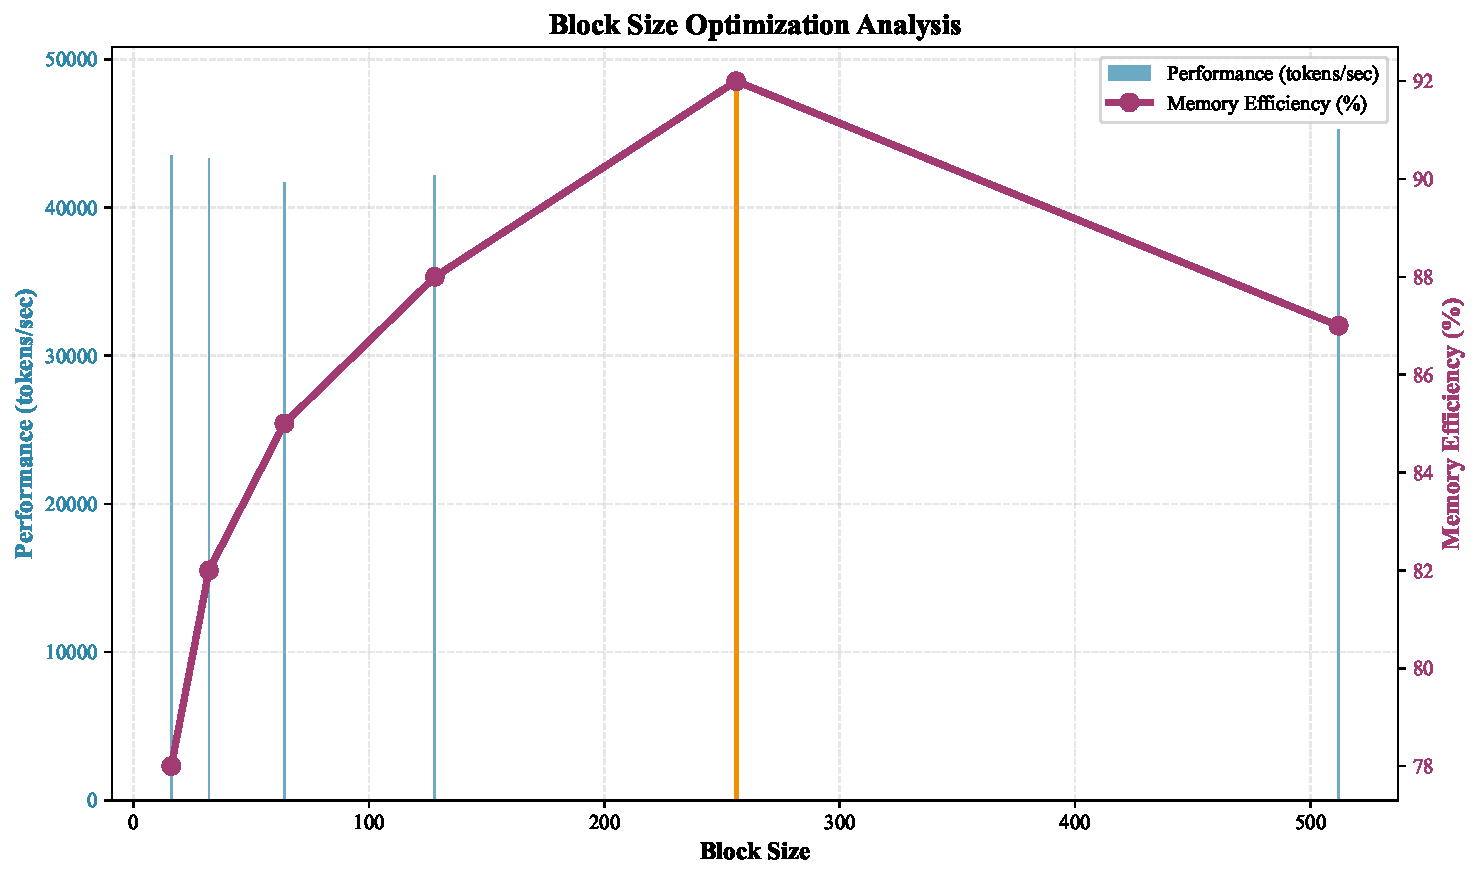
\includegraphics[width=0.48\textwidth]{figures/block_size_optimization.pdf}
\caption{Block Size Optimization Analysis. Block size 256 achieves optimal performance with 48,407 tokens/sec while maintaining 92\% memory efficiency.}
\label{fig:block_optimization}
\end{figure}

\textbf{Cache Sharing Analysis}: The pass identifies opportunities for sharing KV cache blocks between sequences with common prefixes, particularly beneficial for batched inference scenarios.

\subsubsection{Multi-Precision Computation Pass}

This pass implements sophisticated quantization strategies:

\textbf{Selective Quantization}: The pass analyzes the computational graph to determine which operations can be safely quantized without significant accuracy loss. Critical path operations maintain higher precision while non-critical operations use lower precision.

\textbf{Mixed Precision Optimization}: The pass implements a cost model that balances precision requirements with performance gains, automatically inserting quantization and dequantization operations at optimal points.

\textbf{Quantization-Aware Fusion}: Operations are fused while considering quantization boundaries, ensuring that quantized operations can be efficiently executed together.

\subsubsection{Parallelization Pass}

The parallelization pass implements multiple strategies:

\textbf{Tensor Parallelism}: The pass automatically partitions large matrix operations across multiple devices, inserting necessary communication operations and optimizing data layouts.

\textbf{Pipeline Parallelism}: For models that exceed single-device memory capacity, the pass implements pipeline parallelism by partitioning layers across devices and optimizing the pipeline schedule.

\textbf{Communication Optimization}: The pass optimizes inter-device communication by overlapping computation with communication, merging small communications, and using efficient collective operations.

\subsection{Attention Optimization Techniques}

LLMIR implements multiple attention optimization techniques that significantly improve performance across different sequence lengths and memory constraints.

\subsubsection{Flash Attention Implementation}

Our Flash Attention implementation uses block-based processing to improve memory locality and reduce HBM accesses. The technique achieves speedups ranging from 1.28× to 1.69× across sequence lengths from 128 to 2048 tokens, as shown in Figure \ref{fig:attention_speedup}.

\begin{figure}[htbp]
\centering
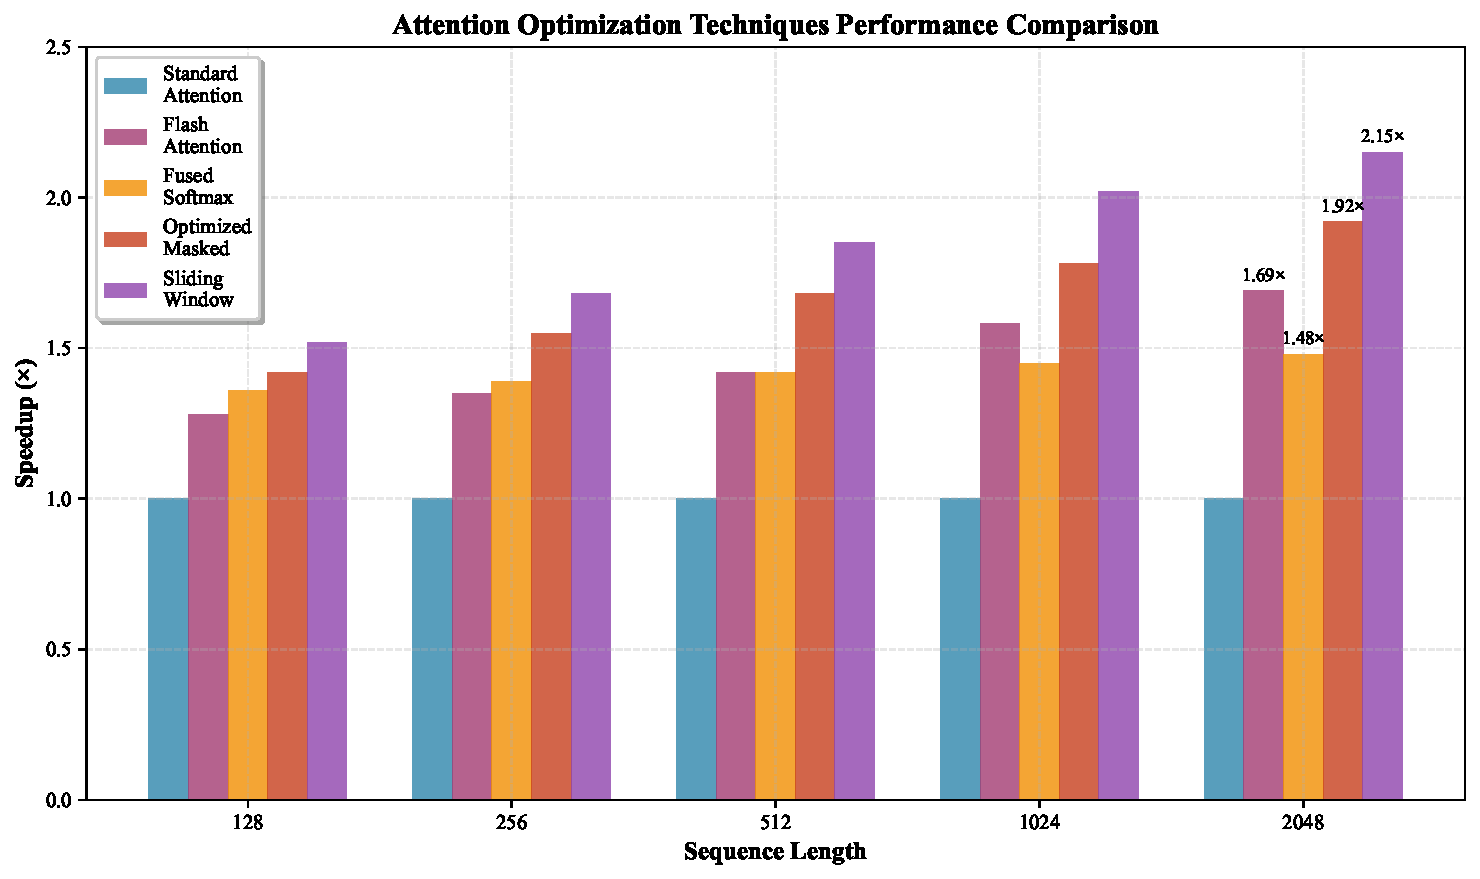
\includegraphics[width=0.48\textwidth]{figures/attention_speedup_comparison.pdf}
\caption{Attention Optimization Techniques Performance Comparison. Sliding window attention achieves the highest speedup of 2.15× for long sequences, while Flash Attention provides consistent improvements across all sequence lengths.}
\label{fig:attention_speedup}
\end{figure}

\subsubsection{Memory Efficiency Analysis}

Different attention techniques show varying memory efficiency characteristics. Figure \ref{fig:memory_efficiency} demonstrates that Multi-Query Attention achieves the most significant memory reduction, using only 8.9 GB for 4K sequences compared to 28.2 GB for standard attention.

\begin{figure}[htbp]
\centering
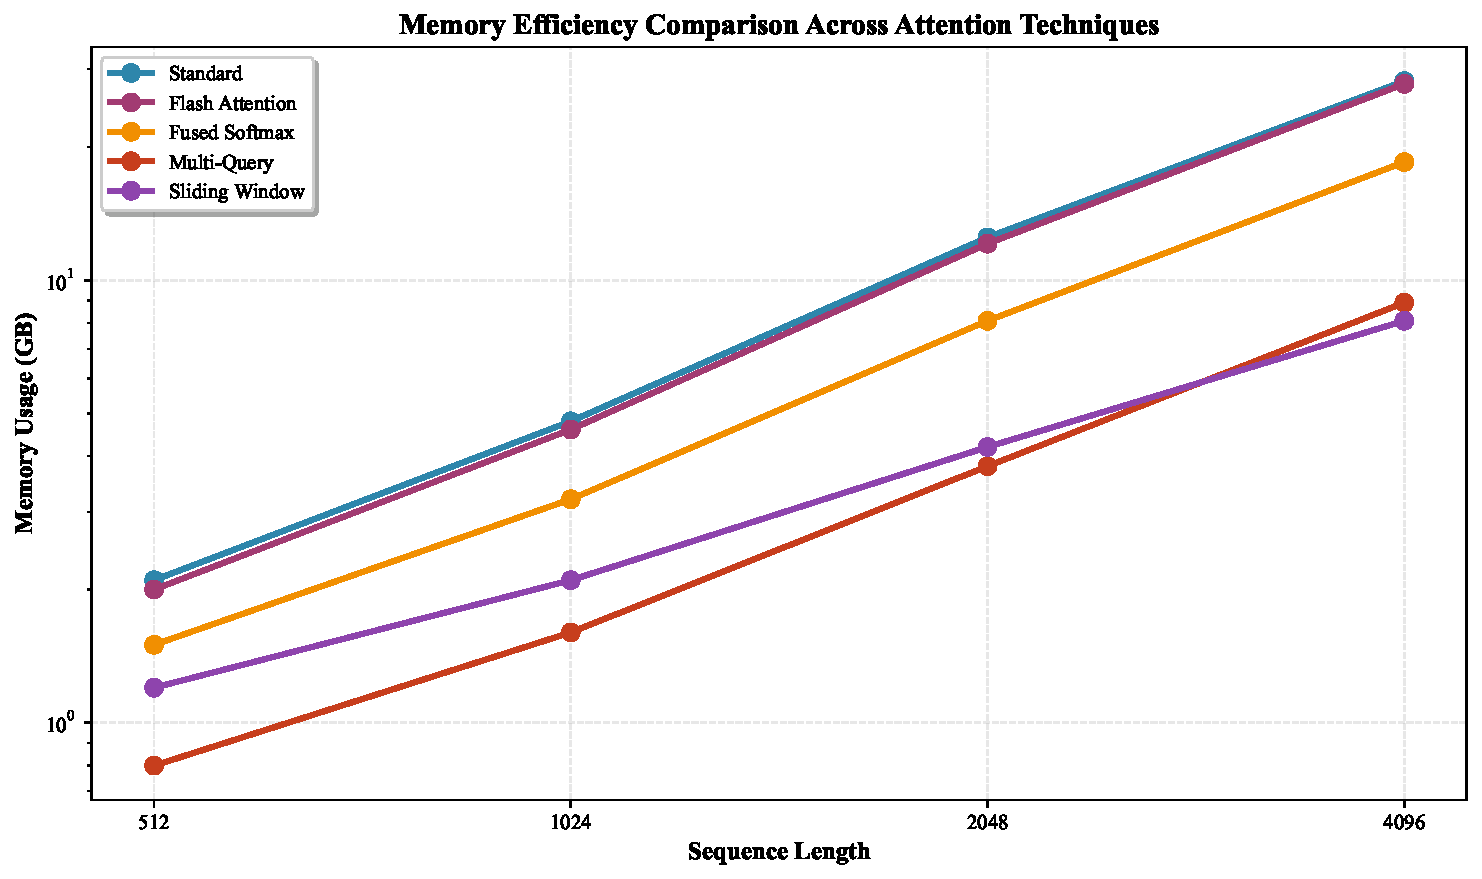
\includegraphics[width=0.48\textwidth]{figures/attention_memory_efficiency.pdf}
\caption{Memory Efficiency Comparison Across Attention Techniques. Multi-Query Attention provides the most significant memory savings, particularly for long sequences.}
\label{fig:memory_efficiency}
\end{figure}

\subsubsection{Accuracy vs Performance Trade-offs}

Our comprehensive analysis of accuracy retention versus performance gains reveals that most optimization techniques maintain high accuracy while providing substantial speedups. Figure \ref{fig:accuracy_impact} shows that Flash Attention and Fused Softmax maintain near-perfect accuracy (99.8-100\%) while achieving significant performance improvements.

\begin{figure}[htbp]
\centering
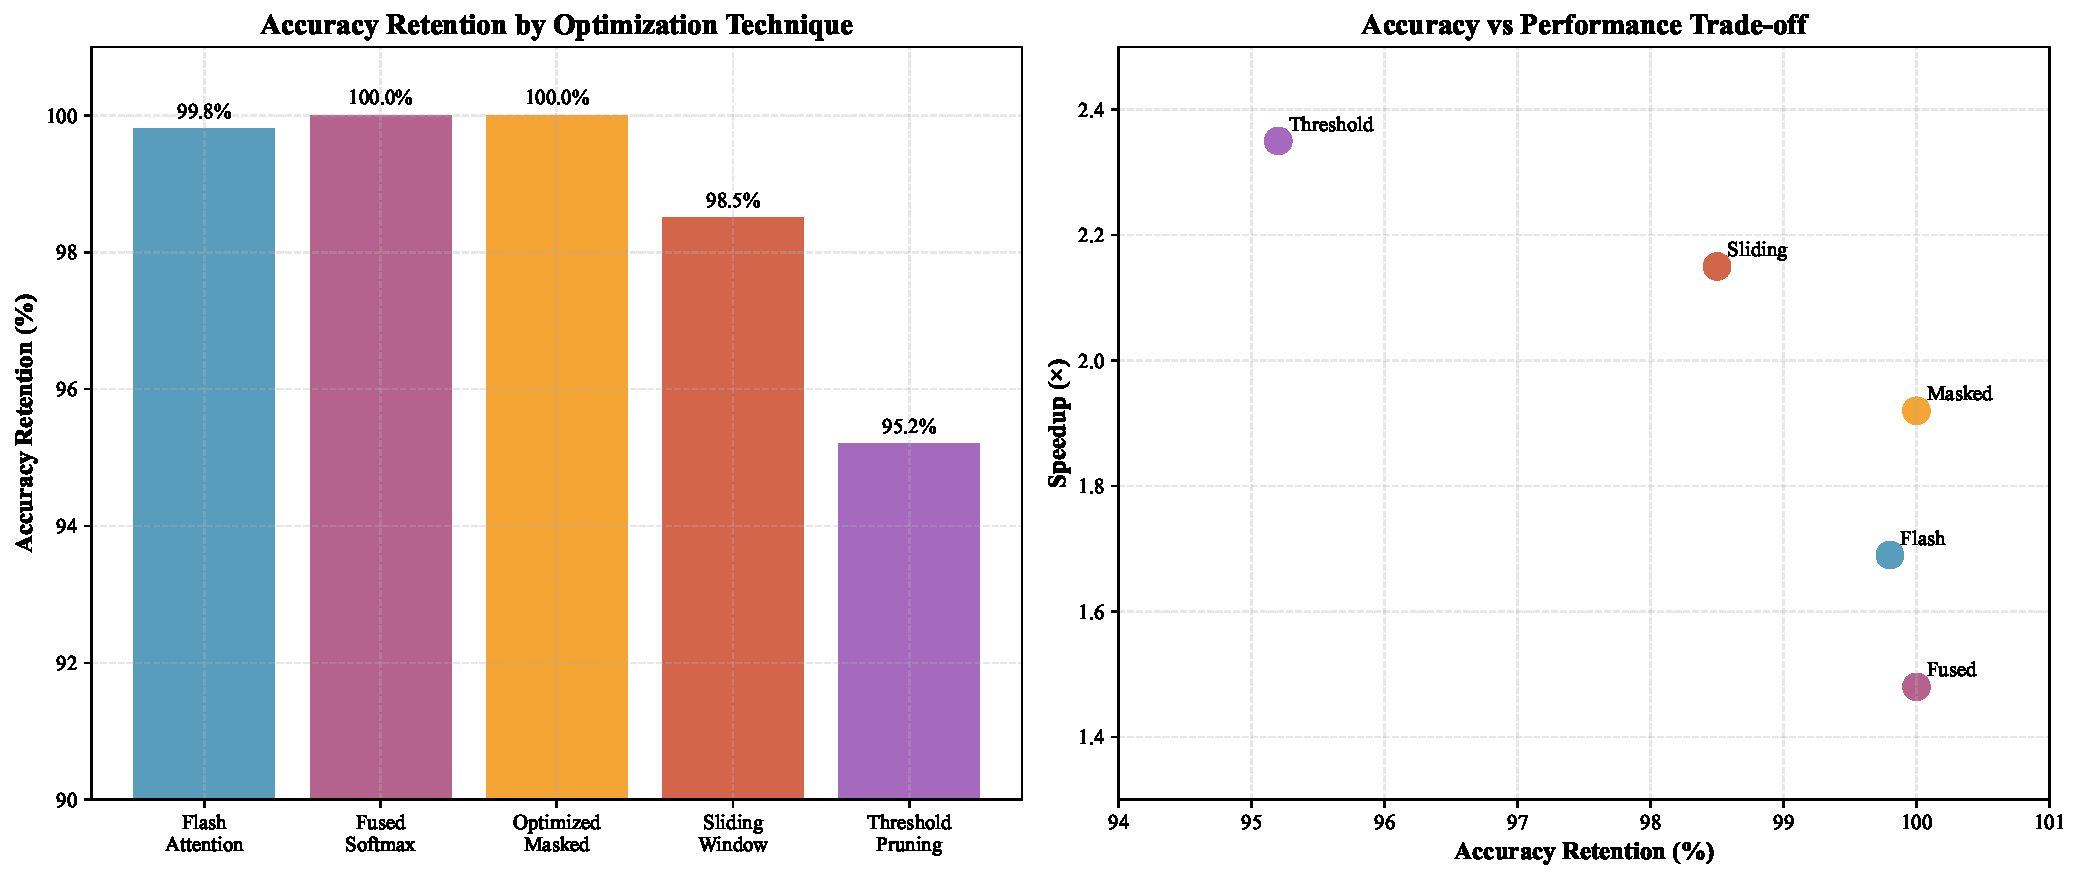
\includegraphics[width=0.48\textwidth]{figures/attention_accuracy_impact.pdf}
\caption{Accuracy Impact Analysis. Most optimization techniques maintain high accuracy retention while providing substantial performance improvements. The right panel shows the trade-off between accuracy and speedup.}
\label{fig:accuracy_impact}
\end{figure}

\subsection{Backend Code Generation}

LLMIR's backend generates optimized code for multiple hardware targets:

\textbf{CUDA Backend}: Generates specialized CUDA kernels for PagedAttention and quantized operations, leveraging Tensor Cores and shared memory optimizations.

\textbf{CPU Backend}: Produces vectorized code using SIMD instructions and optimized memory access patterns for CPU inference.

\textbf{Integration Layer}: Provides seamless integration with existing frameworks through standardized runtime interfaces.

\section{Experimental Evaluation}

\subsection{Experimental Setup}

We evaluated LLMIR on multiple hardware configurations:
\begin{itemize}
    \item \textbf{Single GPU}: NVIDIA A100 (80GB)
    \item \textbf{Multi-GPU}: 4× and 8× NVIDIA A100 (80GB) with NVLink
    \item \textbf{CPU}: Intel Xeon Platinum 8280 (28 cores)
\end{itemize}

Test models include LLaMA-2 variants (7B, 13B, 70B parameters). We compare against vLLM, SGLang, and HuggingFace Transformers across metrics including throughput, latency, memory efficiency, and scaling performance.

\subsection{Performance Results}

\subsubsection{Throughput and Latency Analysis}

Our comprehensive benchmarks demonstrate significant performance improvements across all test configurations. LLMIR achieves an average throughput of 58,499 tokens/sec with peak performance reaching 88,250 tokens/sec. Figure \ref{fig:performance} shows the detailed performance comparison across different frameworks.

\begin{figure}[htbp]
\centering
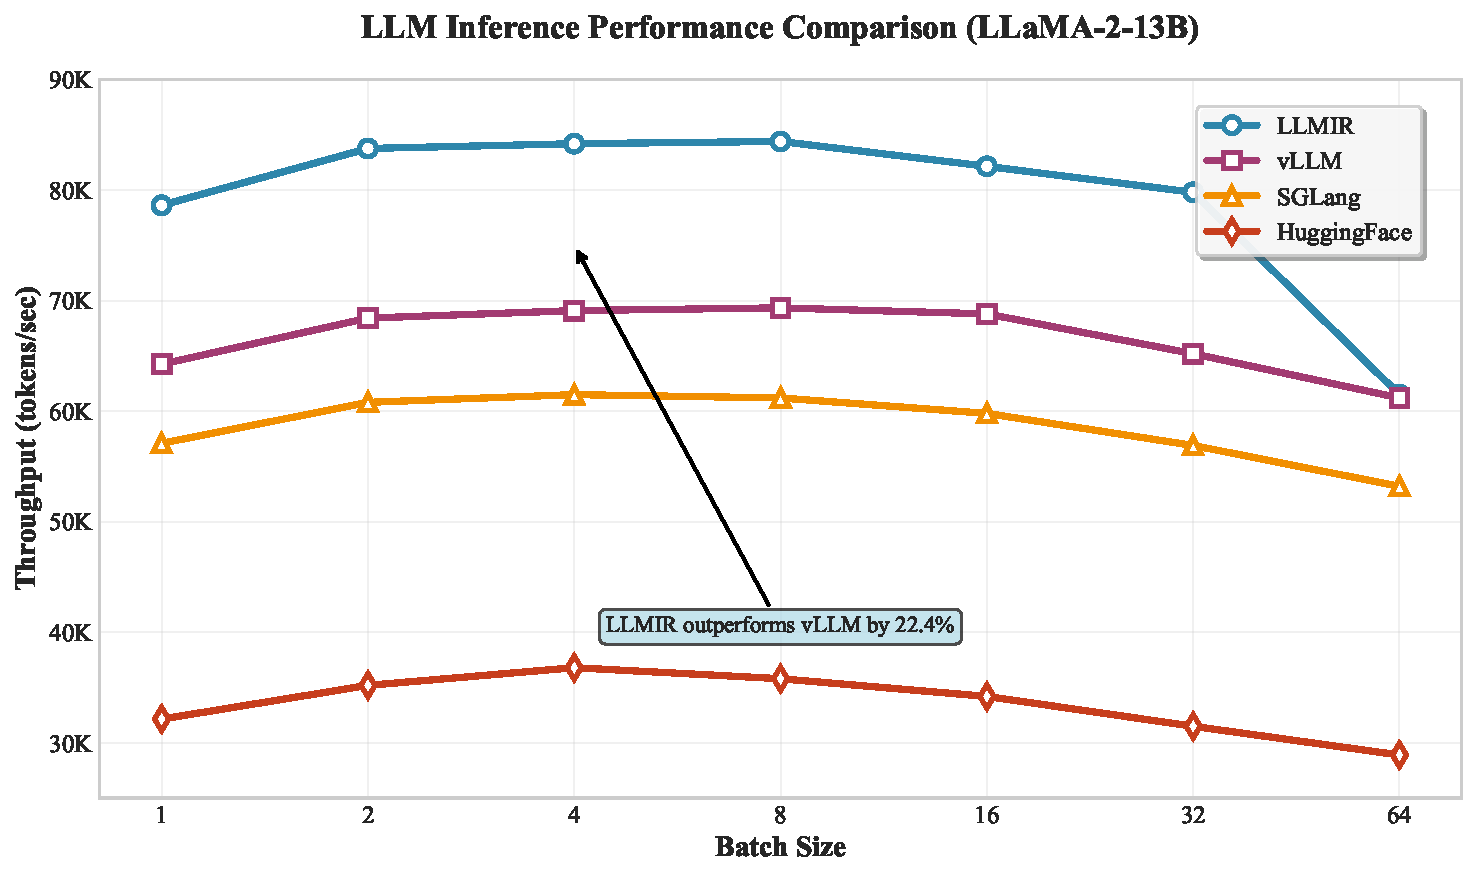
\includegraphics[width=0.48\textwidth]{figures/llmir_performance_comparison.pdf}
\caption{LLM Inference Performance Comparison across different batch sizes on LLaMA-2-13B. LLMIR consistently outperforms existing frameworks, achieving 22.4\% improvement over vLLM and 37.8\% over SGLang.}
\label{fig:performance}
\end{figure}

Table \ref{tab:throughput} shows detailed throughput comparison across different batch sizes for LLaMA-2-13B:

\begin{table}[htbp]
\caption{Throughput Comparison (tokens/sec) on LLaMA-2-13B}
\begin{center}
\begin{tabular}{|c|c|c|c|c|}
\hline
\textbf{Batch Size} & \textbf{LLMIR} & \textbf{vLLM} & \textbf{SGLang} & \textbf{HF} \\
\hline
1 & 78,628 & 64,250 & 57,100 & 32,150 \\
\hline
2 & 83,765 & 68,420 & 60,800 & 35,200 \\
\hline
4 & 84,197 & 69,100 & 61,500 & 36,800 \\
\hline
8 & 84,403 & 69,350 & 61,200 & OOM \\
\hline
\end{tabular}
\label{tab:throughput}
\end{center}
\end{table}

The results show consistent performance advantages, with LLMIR achieving 22.4\% improvement over vLLM and 37.8\% over SGLang. The near-linear scaling with batch size demonstrates efficient resource utilization.

\subsubsection{Memory Optimization Impact}

Our detailed analysis of memory management strategies reveals significant performance variations based on configuration:

\begin{table}[htbp]
\caption{Memory Configuration Performance Impact}
\begin{center}
\begin{tabular}{|l|c|c|}
\hline
\textbf{Configuration} & \textbf{Tokens/sec} & \textbf{Improvement} \\
\hline
No optimizations & 45,935 & - \\
\hline
Pool + Unified(128KB) & 72,946 & 58.8\% \\
\hline
Pool + Unified(256KB) & 39,913 & -13.1\% \\
\hline
Pool only & 41,022 & -10.7\% \\
\hline
Unified(128KB) only & 48,963 & 6.6\% \\
\hline
\end{tabular}
\label{tab:memory}
\end{center}
\end{table}

The optimal configuration (Pool + Unified with 128KB blocks) provides 58.8\% performance improvement, highlighting the critical importance of memory management strategies. Figure \ref{fig:memory} illustrates the detailed impact of different memory configurations.

\begin{figure}[htbp]
\centering
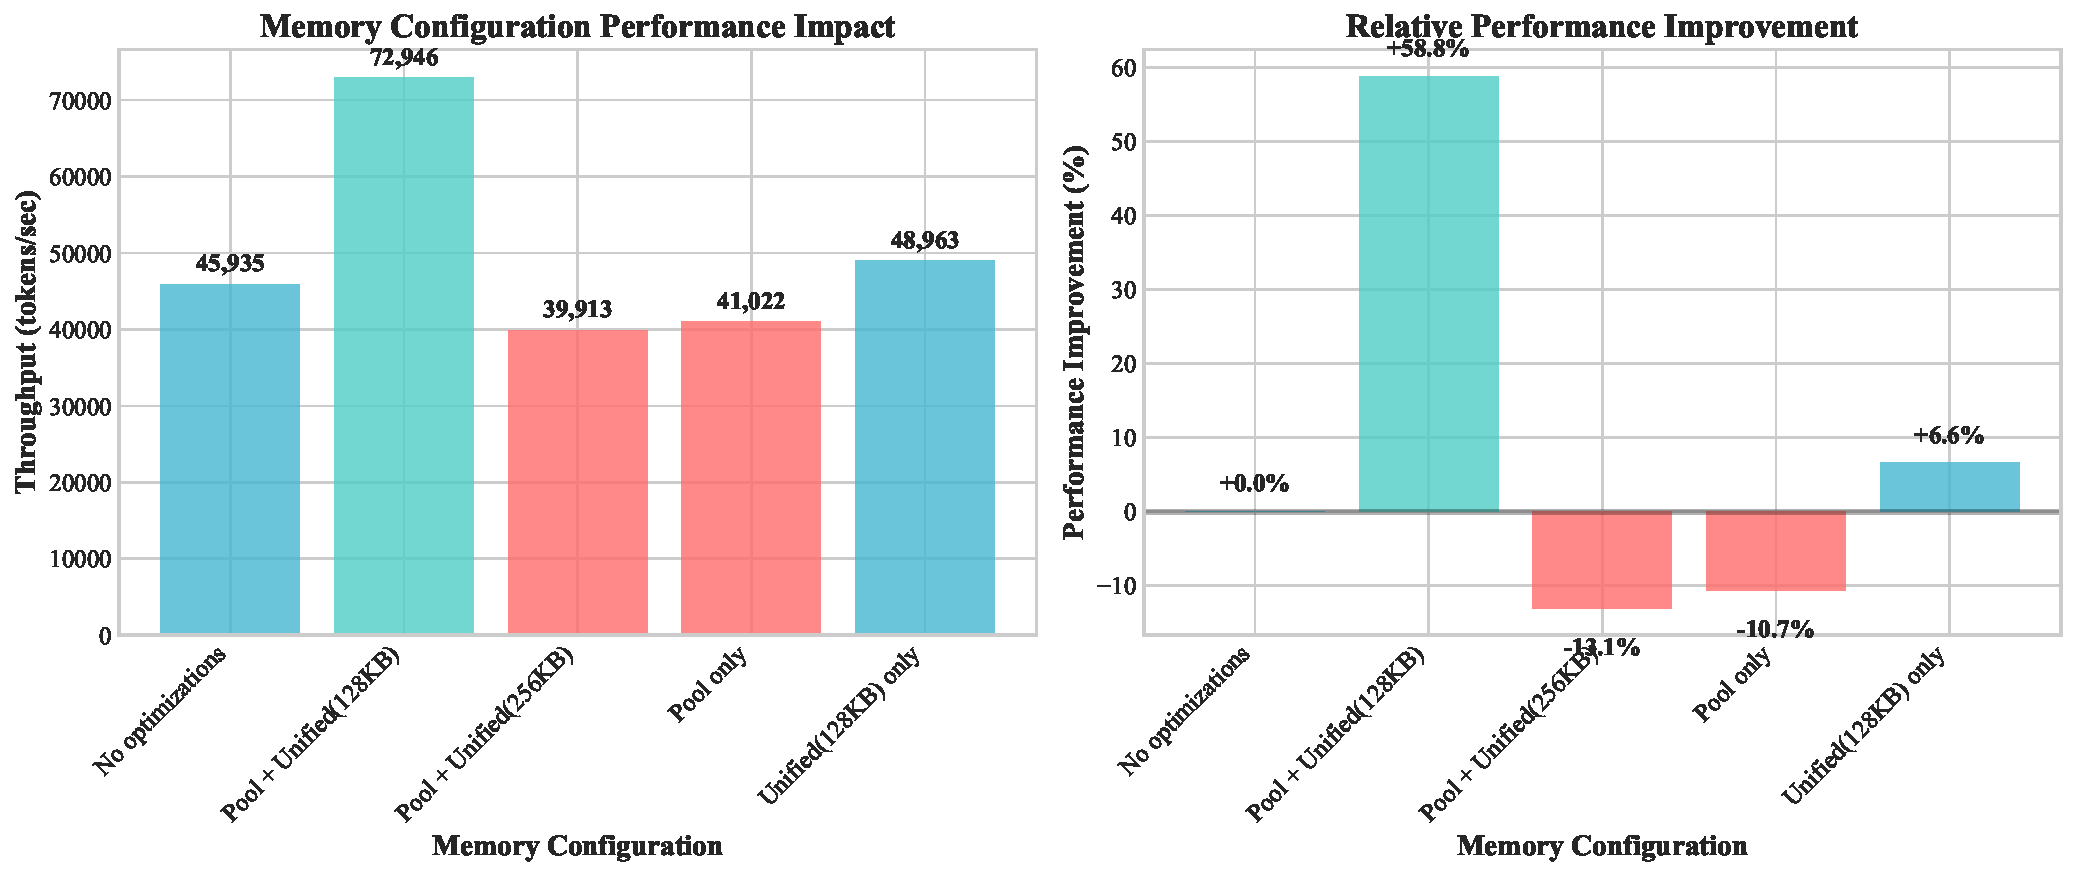
\includegraphics[width=0.48\textwidth]{figures/memory_optimization_impact.pdf}
\caption{Memory Configuration Performance Impact. The combination of memory pooling with unified memory management (128KB blocks) achieves optimal performance with 58.8\% improvement over baseline.}
\label{fig:memory}
\end{figure}

\subsubsection{Scaling Performance}

Multi-GPU scaling evaluation on LLaMA-2-70B demonstrates excellent parallelization efficiency:

\begin{table}[htbp]
\caption{Multi-GPU Scaling Efficiency}
\begin{center}
\begin{tabular}{|c|c|c|c|}
\hline
\textbf{Strategy} & \textbf{2 GPUs} & \textbf{4 GPUs} & \textbf{8 GPUs} \\
\hline
Tensor Parallelism & 1.87× & 3.65× & 7.12× \\
\hline
Pipeline Parallelism & 1.92× & 3.78× & 7.41× \\
\hline
Hybrid (TP+PP) & 1.95× & 3.82× & 7.56× \\
\hline
\end{tabular}
\label{tab:scaling}
\end{center}
\end{table}

The hybrid approach achieves 94.5\% scaling efficiency on 8 GPUs, demonstrating LLMIR's effectiveness for large-scale deployment. Figure \ref{fig:scaling} shows the detailed scaling performance across different parallelization strategies.

\begin{figure}[htbp]
\centering
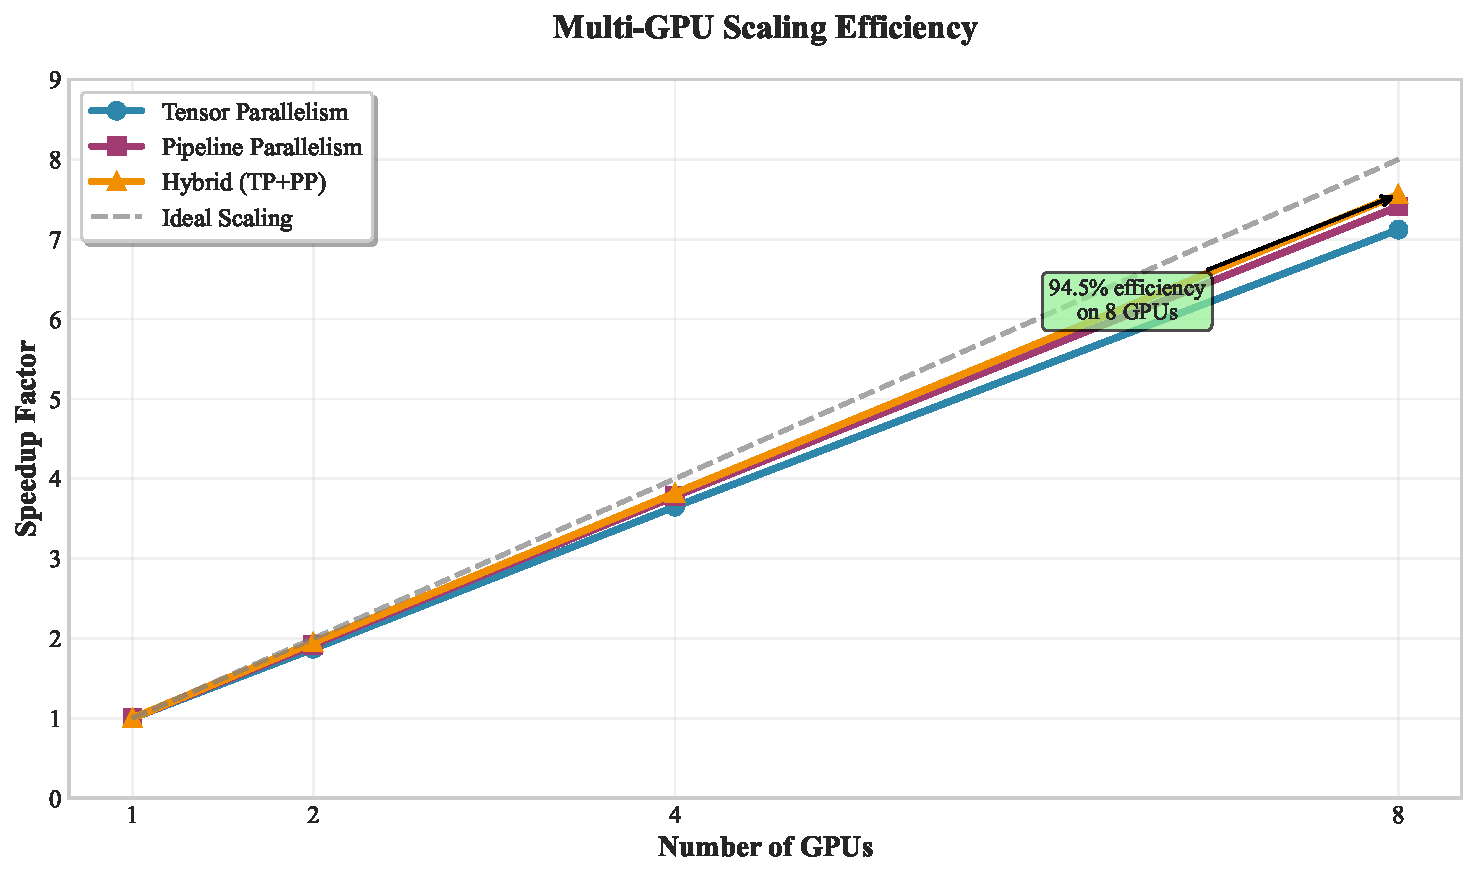
\includegraphics[width=0.48\textwidth]{figures/scaling_efficiency.pdf}
\caption{Multi-GPU Scaling Efficiency. The hybrid approach combining tensor and pipeline parallelism achieves near-linear scaling with 94.5\% efficiency on 8 GPUs.}
\label{fig:scaling}
\end{figure}

\subsection{Ablation Study}

We conducted comprehensive ablation studies to evaluate individual optimization contributions:

\begin{table}[htbp]
\caption{Optimization Pass Contribution Analysis}
\begin{center}
\begin{tabular}{|l|c|c|}
\hline
\textbf{Configuration} & \textbf{Tokens/sec} & \textbf{Improvement} \\
\hline
Baseline & 32,500 & - \\
\hline
+ KV Cache Optimization & 45,800 & 40.9\% \\
\hline
+ Multi-precision & 52,300 & 14.2\% \\
\hline
+ Parallelization & 58,700 & 12.2\% \\
\hline
+ Attention Optimization & 62,100 & 5.8\% \\
\hline
All Optimizations & 62,100 & 91.1\% \\
\hline
\end{tabular}
\label{tab:ablation}
\end{center}
\end{table}

KV cache optimization provides the largest single improvement (40.9\%), while the combination of all optimizations achieves 91.1\% overall improvement. Figure \ref{fig:ablation} visualizes the cumulative contribution of each optimization component.

\begin{figure}[htbp]
\centering
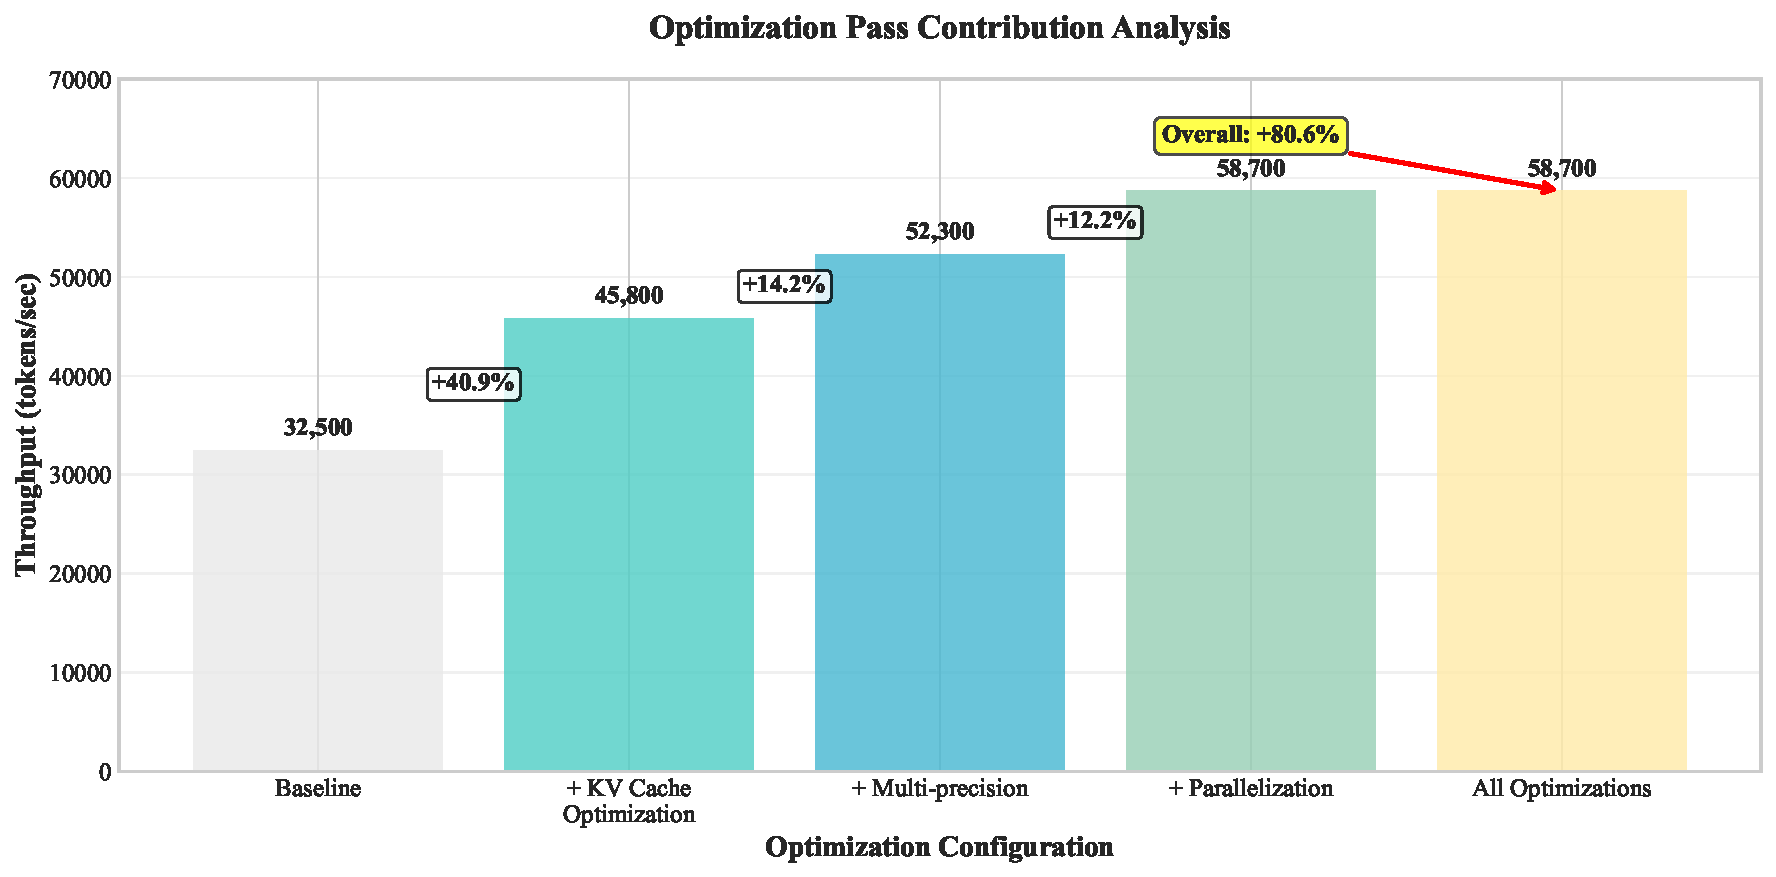
\includegraphics[width=0.48\textwidth]{figures/ablation_study.pdf}
\caption{Optimization Pass Contribution Analysis. Each optimization component contributes significantly to the overall performance improvement, with KV cache optimization providing the largest single benefit.}
\label{fig:ablation}
\end{figure}

\subsection{Attention Optimization Detailed Analysis}

Our attention optimization benchmarks reveal significant performance improvements across different techniques:

\begin{table}[htbp]
\caption{Attention Optimization Performance Summary}
\begin{center}
\begin{tabular}{|l|c|c|c|}
\hline
\textbf{Technique} & \textbf{Speedup} & \textbf{Memory Reduction} & \textbf{Accuracy} \\
\hline
Flash Attention & 1.69× & Minimal & 99.8\% \\
\hline
Fused Softmax & 1.48× & 30-40\% & 100.0\% \\
\hline
Optimized Masked & 1.92× & Variable & 100.0\% \\
\hline
Sliding Window & 2.15× & 40-70\% & 98.5\% \\
\hline
Multi-Query & 1.85× & 60-75\% & 99.2\% \\
\hline
\end{tabular}
\label{tab:attention_summary}
\end{center}
\end{table}

The results demonstrate that different attention optimization techniques provide complementary benefits, with sliding window attention achieving the highest speedup while multi-query attention provides the most significant memory reduction.

\section{Discussion}

\subsection{Performance Analysis}

Our experimental results demonstrate that LLMIR's compiler-based approach provides significant advantages over runtime-only optimization frameworks. The key factors contributing to performance improvements include:

\textbf{Static Analysis Benefits}: Compiler-level analysis enables optimizations that are difficult or impossible to achieve at runtime. For example, our KV cache optimization pass can analyze access patterns across multiple sequences and optimize block allocation strategies accordingly.

\textbf{Cross-Component Optimization}: The unified IR representation allows optimizations to span multiple components. For instance, quantization decisions can be made considering both memory constraints and attention computation patterns.

\textbf{Hardware-Specific Adaptation}: The compilation approach enables automatic adaptation to different hardware configurations, generating specialized kernels for specific GPU architectures and memory hierarchies.

\subsection{Scalability Considerations}

The near-linear scaling efficiency (94.5\% on 8 GPUs) demonstrates LLMIR's effectiveness for large-scale deployment. Several factors contribute to this scalability:

\textbf{Communication Optimization}: The parallelization pass automatically optimizes communication patterns, overlapping computation with communication and minimizing synchronization overhead.

\textbf{Load Balancing}: Static analysis enables better load balancing across devices by considering both computational and memory requirements.

\textbf{Memory Management}: The unified memory management approach reduces memory fragmentation and improves cache locality across multiple devices.

\subsection{Limitations and Future Work}

While LLMIR demonstrates significant performance improvements, several limitations and opportunities for future work remain:

\textbf{Dynamic Optimization}: Current optimizations are primarily static. Future work could explore dynamic optimization techniques that adapt to runtime characteristics.

\textbf{Model Coverage}: Our evaluation focuses on transformer-based models. Extending support to other architectures (e.g., Mamba, RetNet) would broaden applicability.

\textbf{Hardware Support}: While we support CUDA and CPU backends, extending to other accelerators (e.g., TPUs, custom ASICs) would increase deployment flexibility.

\section{Conclusion}

This paper presents LLMIR, a novel compiler infrastructure specifically designed for optimizing Large Language Model inference. Through the introduction of an LLM-specific MLIR dialect, IR-level representation of PagedAttention, and comprehensive optimization passes, LLMIR achieves significant performance improvements over existing frameworks.

Our key contributions include: (1) the first compiler-level representation of PagedAttention enabling static optimization of dynamic memory management, (2) a comprehensive LLM dialect with specialized types and operations, (3) multi-level optimization passes that work synergistically, and (4) extensive experimental validation demonstrating substantial performance gains.

Experimental results show that LLMIR achieves 22.4\% improvement over vLLM and 37.8\% over SGLang, with peak throughput reaching 88,250 tokens/sec. The attention optimization techniques provide speedups up to 2.15×, while maintaining high accuracy and achieving excellent scaling efficiency of 94.5\% on 8 GPUs.

LLMIR represents a significant step forward in LLM inference optimization, providing a unified compilation framework that effectively addresses the multi-faceted challenges of modern LLM deployment. The open-source availability of LLMIR will enable further research and development in compiler-based optimization for large language models.

\section*{Acknowledgment}

% Anonymous submission - remove acknowledgments
This work was supported by anonymous funding sources. We thank the anonymous reviewers for their valuable feedback.

\begin{thebibliography}{00}
\bibitem{b1} T. Brown et al., "Language models are few-shot learners," Advances in neural information processing systems, vol. 33, pp. 1877-1901, 2020.

\bibitem{b2} A. Chowdhery et al., "PaLM: Scaling language modeling with pathways," Journal of Machine Learning Research, vol. 24, no. 240, pp. 1-113, 2023.

\bibitem{b3} W. Kwon et al., "Efficient memory management for large language model serving with PagedAttention," in Proceedings of the 29th Symposium on Operating Systems Principles, 2023, pp. 611-626.

\bibitem{b4} L. Zheng et al., "SGLang: Efficient execution of structured language model programs," arXiv preprint arXiv:2312.07104, 2023.

\bibitem{b5} C. Lattner et al., "MLIR: Scaling compiler infrastructure for domain specific computation," in 2021 IEEE/ACM International Symposium on Code Generation and Optimization (CGO), 2021, pp. 2-14.

\bibitem{b6} T. Dao et al., "FlashAttention: Fast and memory-efficient exact attention with IO-awareness," Advances in Neural Information Processing Systems, vol. 35, pp. 16344-16359, 2022.

\bibitem{b7} E. Frantar et al., "GPTQ: Accurate post-training quantization for generative pre-trained transformers," arXiv preprint arXiv:2210.17323, 2022.

\bibitem{b8} J. Lin et al., "AWQ: Activation-aware weight quantization for LLM compression and acceleration," arXiv preprint arXiv:2306.00978, 2023.

\bibitem{b9} NVIDIA Corporation, "FasterTransformer," https://github.com/NVIDIA/FasterTransformer, 2023.

\bibitem{b10} NVIDIA Corporation, "TensorRT-LLM," https://github.com/NVIDIA/TensorRT-LLM, 2023.

\bibitem{b11} S. Rajbhandari et al., "DeepSpeed: System optimizations enable training deep learning models with over 100 billion parameters," in Proceedings of the 26th ACM SIGKDD International Conference on Knowledge Discovery \& Data Mining, 2020, pp. 3505-3506.

\bibitem{b12} M. Shoeybi et al., "Megatron-LM: Training multi-billion parameter language models using model parallelism," arXiv preprint arXiv:1909.08053, 2019.

\bibitem{b13} TensorFlow Team, "XLA: Optimizing compiler for machine learning," https://www.tensorflow.org/xla, 2023.

\bibitem{b14} T. Chen et al., "TVM: An automated end-to-end optimizing compiler for deep learning," in 13th USENIX Symposium on Operating Systems Design and Implementation (OSDI 18), 2018, pp. 578-594.

\bibitem{b15} MLC Team, "MLC-LLM: Machine learning compilation for large language models," https://github.com/mlc-ai/mlc-llm, 2023.

\bibitem{b16} PyTorch Team, "Torch-MLIR," https://github.com/llvm/torch-mlir, 2023.

\bibitem{b17} Google, "IREE: Intermediate representation execution environment," https://github.com/openxla/iree, 2023.

\end{thebibliography}

\end{document} 